\section{Design and Implementation}
LibSmoke is composed essentially, as told before, by SKNX and AES.\par
\vspace{5mm}
\textbf{Secure KNX - }Allows the user to create the \emph{backend} connection between different devices, in particular in this paper/project we have considered the LinuxTCP one. It includes also a \emph{pktwrapper} that handles the packets exchange : splitting data in pkts of 15 bytes payload and recomposing next them together. There are also available multiple KeyExchange algorithms that allows to calculate a shared key; we have here test the \emph{mka} (Multi-party Key Agreement Algorithm).\par
\vspace{5mm}
\textbf{AES256\_CTR - }Given that \emph{mka} returns a key of 32 bytes we choose AES256, but in the \emph{AES Library} there are also available AES128 and AES192. It includes all the implementations of AES ECB, CTR and CBC, in particular we use CTR cause it also provides padding.\par
\vspace{5mm}
Given this background we decide to split LibSmoke in 2 classes : ClientSmoke and ServerSmoke.

\vspace{0.5cm}
\begin{figure}[h]
	\centering
	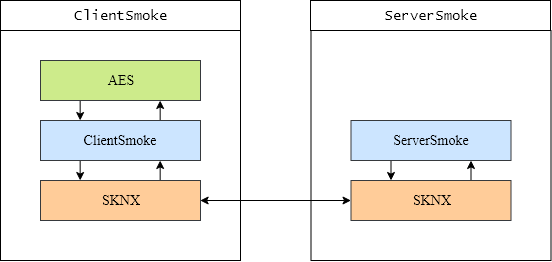
\includegraphics[scale=0.5]{Images/Diagrams/Architecture}
	\caption{LibSmoke Architecture}
\end{figure}
\vspace{0.2cm}

\newpage
\textbf{ClientSmoke - }Initialized by devices that needs to send and receive pkts, given also the functionality to encrypt and decrypt data with the encryption algorithm [AES256\_CTR].

\begin{lstlisting}[language=C++, caption={ClientSmoke}]

\end{lstlisting}